\documentclass[tikz, border=10pt]{standalone}
\usepackage{tikz-cd}
\usepackage{tikz}

\usetikzlibrary{arrows,automata,positioning}

\begin{document}

  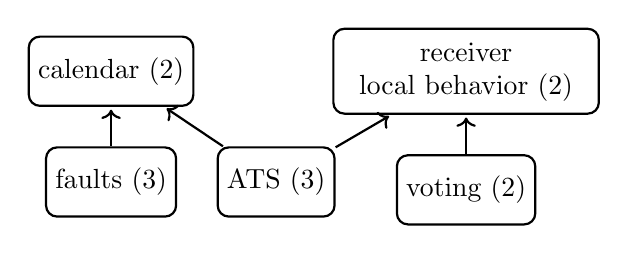
\begin{tikzpicture}[->, node distance=2.6cm, auto, shorten >=1pt, bend angle=45,thick]
    \tikzstyle{every state}=[rectangle, rounded corners]

    \node[state] (calendar) {calendar (2)};
    \node[state] (lieutenant) [right=1.75cm of calendar]
        {\begin{tabular}{c}receiver\\local behavior (2)\end{tabular}};
    \node[state] (faults) [below=0.5cm of calendar] {faults (3)};
    \node[state] (asm) [right=0.5cm of faults] {ATS (3)};
    \node[state] (voting) [below=0.5cm of lieutenant] {voting (2)};

    \tikzstyle{every node}=[]

    \path
    (faults) edge [] node {} (calendar)
    (asm)    edge [] node {} (calendar)
    (asm)    edge [] node {} (lieutenant)
    (voting) edge [] node {} (lieutenant);

  \end{tikzpicture}

\end{document}
